\hypertarget{introduction}{%
\section{Introduction}\label{introduction}}

Designing and operating chemical factories requires accurate,
comprehensive models of their behaviour. With the advent of more
computing resources and networked sites, process modelling has become
more critical than ever before. One way this is shown is in the rise in
popularity of Digital Twins, which aim to make a complete and
comprehensive model of many different properties of entire sites and
their surroundings \citep{walmsley2024adaptive}. 

A powerful tool to represent processes is equation-oriented algebraic
modelling, as processes often closely follow first-principles behaviour
and include non-linear dynamics, two things that equation-oriented
modelling excels at \citep{shacham1982equation}. At its simplest,
equation-oriented modelling involves specifying equations to represent
the system, and solving those equations to find the unknown properties.
This is very flexible which makes it a powerful tool to build Digital Twins.
However, the comprehensiveness of a digital twin naturally leads to very complicated models.
This results in very complex equation-oriented models (EOMs) and very
large sets of equations.

EOMs are usually specified in a declarative manner through Algebraic
Modelling Languages (AMLs), such as GAMS \citep{robichaud2010introduction}, 
AMPL \citep{fourer1990ampl}, Pyomo \citep{hart2011pyomo}, and JuMP \citep{lubin2023jump}. To help models remain understandable,
AMLs apply software engineering principles of abstraction
and encapsulation so that the entire system does not always have to be
considered at once. This often means the person using the model does not
directly interact with the equations behind it. They may not
know what is the best way to specify all
degrees of freedom in the model. Combining multiple models and adding additional
constraints further complicates the issue.

This article focuses on a modelling workflow and software abstraction
for specification management in EOMs. We propose that the model developer should
explicitly encode specification intent: which variables in the model are
design variables, which are operating variables, and which are dependent
variables. Design and operating variables are fixed by default. As
required, design and operating variables can be replaced by dependent
variables in the equation-oriented model.

We refer to the resulting structure as a model's specification topology:
the relationship between the variables fixed by default and the
variables that may replace them for a particular study. This topology is
often managed informally in practice, but is not usually represented
explicitly in equation-oriented modelling frameworks. By making it
explicit, the AML can better preserve specification consistency and it
becomes easier to build tools on top of the modelling framework to help
with model construction, interpretation, and initialisation.

Our library, pyomo-replace, demonstrates these ideas in the Pyomo and
IDAES \citep{miller2018next} ecosystem, and the Ahuora Platform
provides a case study of this structured specification-management
approach in a graphical application.

\hypertarget{literature-review}{%
\subsection{Context}\label{literature-review}}

\hypertarget{equation-oriented-modelling}{%
\subsubsection{Equation-oriented
Modelling}\label{equation-oriented-modelling}}

Fundamentally, an EOM is simply a set of mathematical equations.

\[
\begin{aligned}
\quad 
& \{c_i(x) = 0 : i = 1,...,m\} \\
& x \in X.
\end{aligned}
\]

The main parts of these equations are:

\begin{itemize}
\tightlist
\item
  \emph{Variables}:\(x\) represents a set of real numbers we do not know
  ahead of time, but solve the set of equations to find.
\item
  \emph{Constraints:} equality equations that are used to implicitly
  define the value, or solution space of, the variables. \(c_i\)
  represents a constraint expression that must equal zero for \(x\) to
  be considered a valid solution
\end{itemize}

\hypertarget{equation-oriented-modelling-frameworks}{%
\subsubsection{Equation-oriented Modelling
Frameworks}\label{equation-oriented-modelling-frameworks}}

Variables and constraints are fundamentally all that is
required in a mathematical model. However, AMLs introduce layers of 
abstraction for easier programmatic creation and
manipulation of models, borrowing from conventional software development
data structures. A common method is to group variables and 
constraints into a reusable component. This is called a \textit{block} in Pyomo \citep{hart2011pyomo}, or a 
\textit{model} in GPROMS \citep{amador2019introduction}. 


\hypertarget{squaring-a-model}{%
\subsubsection{Squaring a model}\label{squaring-a-model}}

A model that has more unknowns than constraints is said to have \(n\)
degrees of freedom, where \(n_{\text{degrees\ of\ freedom}}\) is given
by

\[
n_{\text{degrees\ of\ freedom}} =  n_{\text{variables}} - n_{\text{constraints}}
\]

In order to solve a set of equations exactly, a ``square'' model is
required, with zero degrees of freedom.

When building an EOM, the user will invariably come across
the problem of Degrees of Freedom; usually they will not have specified
the model sufficiently to be able to solve for an exact solution, i.e
\(n_{\text{degrees\ of\ freedom}} > 0\). Identifying how many and which
variables need to be ``fixed'' to make the model square can be a
challenge \citep{luyben1996design}.

There are a number of techniques to make it easier to square a model.
One simple way is to include documentation about what typical fixed
variables are; this provides a starting point for a modeller that is
piecing together submodels developed by others. There are also automatic
methods to calculate the number of degrees of freedom via static
structural analysis, by subtracting the number of constraints from the
number of variables.

In \citep{bunus2001debugging}, a method is proposed to help debug when a
model is structurally singular by using Dulmage-Mendelson Decomposition to identify
sets of constraints that are over-constrained or under-constrained.
These methods are commonly used in frameworks such as IDAES to help
ensure a square model is valid \citep{lee2024model}. However, while
these techniques are applicable to an entire ``flat'' system of
equations, it is hard to apply them to an individual subsection of a
model without understanding of what external constraints are applied.
Some preliminary work has been conducted to show that in some cases
issues can be identified in this level \citep{nilsson2008type}, but it
is limited in its ability to detect errors and does not appear to have
much uptake in systems such as Pyomo. Additionally, while Dulmage-Mendelson
Decomposition provides a list of over-constrained or
under-constrained components, it does not provide any insight into
which one of them should be constrained.

Much of the research on squaring a model focuses on \emph{if} a model
has degrees of freedom or is fully specified, and \emph{where} the model
is over-specified. There is less research into \emph{why} the model is
over or under specified and \emph{what} a more sensible choice should
be. The problem of squaring a model has not often been analysed within
the domain that the models are used.

Taking a step back to look at the larger picture, Luyben et. al
\citep{luyben1996design} observed and discussed the correlation between
degrees of freedom in design-time models and in control models,
especially for reactors and distillation columns. This is because the
things you specify in design time, such as inlet flow rates or outlet
temperatures, need to be controlled in the real factory, usually by
valves. They argue that calculating the number of controlled parameters
in a plant is an easier way to understand the degrees of freedom of a
process than by trying to analyse the number of equations and variables
in a model that can be adjusted independently.

This is also how many sequential modular models allow a user to set something
that the model would otherwise calculate. The simplest example of this is the 
Goal Seek feature in Excel \citep{microsoft_goalseek_support}.
Aspen Plus uses the Design Spec feature to allow an input to be manipulated to
reach a target output, simulating the steady state effect of a controller \citep{aspenplus111_userguide}.
This can be used with both sequential modular and equation-oriented models, 
but is not required for equation-oriented models as they are implicitly defined. 
Similar features are available in other process modelling software such as gPROMS and DWSIM
\citep{amador2019introduction} \citep{tangsriwong2020modeling}.

\hypertarget{initialising-a-model}{%
\subsubsection{Initializing a model}\label{initializing-a-model}}

Because of the non-linear nature of many EOMs, providing a good initial guess
is often required to find a sensible solution. There are many methods for this,
including warm starts from a previous solution, linear or simplified approximations,
solving initially at a simpler point, or structural decomposition \citep{SAFDARNEJAD201539}.

The exact method often depends on the model structure. The IDAES process modelling framework
defines a separate initialisation routine for each unit model that is added \citep{lee2021idaes}. However, as there
are so many different ways of fully specifying a unit model, these initialisation methods quickly become complicated
as they try to handle many different cases. Even so, if a user chooses to fully specify 
the model in a way that the initialisation method does not expect, it may fail. 
There is a need for more generalisable initialisation methods that can be used regardless of how the model is fully specified.

\hypertarget{methods-of-modelling}{%
\subsubsection{Process Modelling use cases}\label{methods-of-modelling}}

Process models are typically used for one of two main purposes: design and operation \citep{pistikopoulos2021process}.  
In design, the model is used to find the design variables that meet the process requirements. An example of this is sizing of heat exchangers to target a specific heat transfer rate.
It can also be used for performance rating of a given fixed design under different conditions. This can be used as a validation method to check that the design is still suitable when it is not running under the normal optimal conditions.

In operation, the model may used to find the optimal operating conditions for a process, 
such as the flow rate of a valve or the duty of a heater. These can be the targets of a control system, or used for model predictive control. It may also be used to find the current state of the system, particularly to estimate properties that cannot be directly measured. Another use case is to estimate the effect of a change in an operating variable on the rest of the process.

All of these cases require the model to be fully specified, but the choice of which variables to specify differs. A design model may calculate optimal values for design variables, such as heat exchanger area, but in a performance rating study or an operating model, these variables should be fixed. In operating models, if you are estimating the effect of changes to operating variables, then these should also be fixed. If you are trying to find the optimal operating conditions, then these should be unfixed and calculated by the model based on some other target conditions.

While there are certain categories of variables that are typically fixed in different use cases, it can be hard to know which variables to unfix when design variables need to be fixed, or vice versa. The same is true for operating variables. 

\hypertarget{method}{%
\section{Materials \& Methods}\label{method}}

The implicit formulation of EOMs means there is much freedom in how
they are defined. However, that same expressiveness makes it harder to
reason about specification structure or automate parts of model
construction such as initialisation. When multiple EOMs are combined
using principles of abstraction, this challenge compounds.

Our aim is therefore not to alter the mathematics of the underlying
model, but to add an explicit layer for structured specification
management. In software systems, restricting how an interface may be
used can make behaviour easier to understand and automate. We apply the
same idea here to model specification.

We propose that each submodel be defined in a specific way:

\begin{itemize}
  \item a set of `Canonical Variables' are fixed by default, such that the submodel has zero degrees of freedom, and all other variables are defined in terms of these Canonical Variables. These Canonical Variables are either design variables or operating variables in a process model.
  \item if a user wants to fix a variable that is not a Canonical Variable, they must choose a Canonical Variable to unfix, and replace it with one of the dependent variables they want to fix.
  \item if a Canonical Variable is unfixed, an initial guess must be provided for it.
\end{itemize}

In essence, we manage specification as if the EOM exposed an explicit
interface, even though the underlying model remains implicit. The goal
is to make specification changes interpretable and automatable at the
workflow level rather than to reformulate the model itself.

This leads to some helpful emergent properties that make modelling
large systems easier. The manual burden of degree-of-freedom management
is reduced because the Canonical Variables fully define the baseline
specification, and for any additional variable that is fixed, a design
or operating variable is unfixed to preserve the specification count.
Initialisation becomes easier, as initialisation methods only need to be
defined for the Canonical Variables. To convert a model from a design to
operation to performance-rating study, the modeller can remove
replacements on the design or operating variables to re-fix them while
maintaining a fully defined model.

\hypertarget{formal-definition-of-variable-replacement-methodology}{%
\subsection{Formal Definition of Variable Replacement
Methodology}\label{formal-definition-of-variable-replacement-methodology}}

This section provides an operational formalisation of Variable
Replacement, borrowing terminology and concepts from the Pyomo
equation-oriented modelling ecosystem. The purpose is not to present a
complete mathematical theory of solvability or structural analysis.
Rather, it gives a lightweight description of the bookkeeping required
to manage specifications consistently in practice.

\hypertarget{mathematical-definition}{%
\subsubsection{Mathematical Definition}\label{mathematical-definition}}

We represent an EOM operationally as

\[
\mathcal{M} = (\hat{x}, C, F)
\]

where:

\(\hat{x} = (x_1,...,x_n )\) is a vector of \(n\) variables
\(\hat{x} \in \mathbb{R}^n\),

\(C = \{c_i: i = 1,...,m\}\) is a set of \(m\) functions such that
\(c_i(\hat{x}) = 0\) describes the equation-oriented model,

\(F = \{f_i: i \in S \}, S \subseteq \{1,...,n\}\) is an additional set of
functions of the form \(f_i(\hat{x}):= x_i - \bar{x}_i\), representing
the current specification by fixing variable \(x_i\) to the value
\(\bar{x_i}\).

The corresponding specified system is

\[
\{c(\hat{x}) = 0 \; \forall c \in C,\; f(\hat{x}) = 0 \; \forall f \in F\}.
\]

In this paper, \(F\) should be understood as specification metadata
expressed in equation form. We do not claim that the cardinality of
\(C\) and \(F\) alone is sufficient to establish well-posedness,
independence, structural nonsingularity, or feasibility for every
possible EOM. Those issues still depend on the underlying model and are
handled using standard modelling and diagnostic tools.

\hypertarget{degrees-of-freedom}{%
\subsubsection{Degrees of freedom}\label{degrees-of-freedom}}

For operational purposes, we use the usual counting heuristic

\[
\text{DoF} = |\hat{x}| - |F| - |C| 
\]

that is, the number of variables minus the number of fixed variables
minus the number of constraints. This is used here as a practical guide
for specification management, not as a rigorous certificate of
solvability. In particular, zero counted degrees of freedom does not by
itself rule out redundancy, algebraic degeneracy, structural
singularity, or nonlinear infeasibility.

\hypertarget{replacement}{%
\subsubsection{Replacement}\label{replacement}}

Variable replacement is a method of changing which variables in the
model are fixed. We start with a fully defined model
\(\mathcal{M} = (\hat{x}, C, F)\) such that:

\[
DoF(\mathcal{M}) = |\hat{x}| - |F| - |C|  = 0
\]

Suppose we want to fix a new variable \(x_i\). Operationally, this means
adding a new specification equation \(f_i\) to \(F\), giving
\(F' = F \cup \{f_i\}\). On the counting heuristic above,
\(DoF((\hat{x},C,F')) = -1\), indicating that the model is now
over-specified.

To maintain the previous specification count, we also choose an
existing specification equation \(f_j \in F\) to remove. This gives a
new specification set

\[
F_{new} = (F \backslash \{f_j\}) \cup \{f_i\}
\]

and a new operational description

\[
\mathcal{M}_{new} = (\hat{x},C,F_{new})
\]

that restores the counted degrees of freedom to zero.

Note that choosing a suitable \(f_j\) still requires domain knowledge
or structural diagnostics to avoid a poor or infeasible specification.
Variable Replacement does not remove that requirement; it makes the
replacement step explicit and traceable.

\hypertarget{repeated-replacement}{%
\subsubsection{Repeated Replacement}\label{repeated-replacement}}

As the result of a replacement is still an EOM, the process can be
repeated. Each time it is repeated, \(\mathcal{F}_{i}\) is updated to
\(\mathcal{F}_{i+1}\). This gradually replaces the original set of
fixed variables (\(\mathcal{F}\), also called the Canonical Variables)
with a new set of fixed variables (\(\mathcal{F}_{replaced}\)).

\hypertarget{initialisation-of-repeated-replacement}{%
\subsubsection{Initialisation of Models}\label{initialisation-of-repeated-replacement}}

Initialisation methods can be written to calculate initial values for
all variables based on the canonical set of fixed variables
\(\mathcal{F}\). After the initialisation method is run, the model can
be solved with the new set of fixed variables \(\mathcal{F}_{replaced}\)
to calculate the correct values of any variables that were originally
fixed. This allows the same initialisation method to be used regardless
of which variables are fixed as long as an initial guess is provided for
the Canonical Variables.

\hypertarget{design-and-operation-variables}{
\subsubsection{A method for switching between design, performance rating, and operation case studies}\label{design-and-operation-variables}}

In a design case, the design variables can be replaced by dependent variables. This allows a modeller to design a process that meets target conditions. In a performance rating scenario, the design is fixed. Since the model has already defined which variables are design variables, and there is a link between each design variable and the dependent variable replacing it, it is easy to switch between design and performance rating by simply removing the replacements on the design variables. This will still maintain a fully defined model.

Replacing an operating variable with a dependent variable models the effect of a control system on the operating variable when the control system is working effectively. However, those replacements can be removed to model the effect of a change in an operating variable on the rest of the process. This again maintains a fully defined model. Thus, variable replacement allows a modeller to easily switch between design, performance rating, and operation case studies with minimal effort.


\hypertarget{introduction-to-pyomo-replace}{%
\subsection{
Pyomo-replace: A Library for Variable Replacement in Equation-Oriented Models}\label{introduction-to-pyomo-replace}}

To aid in evaluating the advantages of a variable replacement approach
to equation-oriented modelling, we have created a small python package
built on IDAES and pyomo, called pyomo-replace. It keeps track of the Canonical Variables
in an IDAES model, and what variables are replacing them. The list of
Canonical Variables and replacements can be easily printed to the screen to
help explain the model structure.

In Pyomo, an EOM is specified as a set of Blocks, with each block
containing variables and constraints between variables. A Block may
contain Ports, which provide a method of connecting Blocks together.

A Port is simply a collection of variables on a block. A port is
specified to be either an Inlet Port or an Outlet Port. An Inlet port
may be connected to an Outlet port containing an equivalent collection
of variables. The inlet and outlet port do not need to be on the same
block. Connecting two ports creates an equality constraint between the
variable on the Outlet and the variable on the Inlet, that is, the
variable on the inlet is defined to be equal to the corresponding
variable on the outlet port.

The IDAES framework makes it easy to model chemical engineering problems
in pyomo. An equation-oriented model typically represents a chemical
flowsheet, a Block typically represents a unit operation, and Inlet and
Outlet Ports represent inlets and outlets of a unit operation.
Pyomo-replace is specifically targeted to representing these types of
EOMs.

\hypertarget{state-variables}{%
\subsubsection{Canonical Variables}\label{state-variables}}

Because each block contains a set of variables and constraints, it can
be considered an independent system of equations.
Thus, each block has its own set of Canonical Variables that are fixed by default to make it a square model.

The Canonical Variables are chosen by first fixing all inlet variables. By
convention, all inlet variables are automatically considered state
variables, if and only if the inlet is not connected to an outlet. Then,
additional variables are fixed in the model until the model is square.
These variables are also considered Canonical Variables.

The set of Canonical Variables is defined by the author of
the block. This means that if a user imports a block from an external library,
it comes with a predefined set of Canonical Variables and initialisation methods that work with them.
This provides a form of self-documentation and makes it easier to use
external models.

\hypertarget{building-a-model}{%
\subsubsection{Building a model}\label{building-a-model}}

In IDAES, a model is built from a number of blocks. By default, all
Canonical Variables are fixed, and all unconnected inlets are fixed, and so
there will be no degrees of freedom. This fully specifies the model, as
all operations are fully defined: either explicitly, or based on the
outlet conditions of other operations.

\hypertarget{replacing-variables.}{%
\subsubsection{Replacing Variables.}\label{replacing-variables.}}

Once a model is built, different variables can be fixed instead of the
Canonical Variables. For this to happen, a couple of conditions need to be
met:

\begin{itemize}
\tightlist
\item
  A variable must be chosen (that is not already fixed) and fixed. As
  the model was previously fully defined, this will make the model
  over-defined, with -1 degrees of freedom.
\item
  To prevent the model becoming over-defined, a Canonical Variable must be
  chosen and unfixed. We say the Canonical Variable has been ``replaced''
  with the new variable.
\item
  The Canonical Variable must be chosen such that all equations in the model
  are not structurally singular. This can be done by choosing a state
  variable that is part of the Dulmage-Mendelson Over-constrained set 
  when the new variable was fixed \citep{lee2024model}.
\end{itemize}

Metadata about which variables are replacing which Canonical Variables is
stored, for initialisation and interpretation purposes.
If a variable is ever unfixed, the Canonical Variable it replaced
must be fixed again.


\hypertarget{special-cases-for-integrating-pyomo-replace-with-the-idaes-framework}{%
\subsection{Special cases for integrating Pyomo-Replace with the IDAES
Framework}\label{special-cases-for-integrating-pyomo-replace-with-the-idaes-framework}}

In pyomo-replace, to integrate with the pyomo framework we have had to
support indexed variables, networks of blocks, tear guesses, and
optimisation. This section discusses how these higher-level abstractions
impact the application of variable replacement in the domain of chemical
simulation problems.

\hypertarget{indexed-variables}{%
\paragraph{Indexed Variables}\label{indexed-variables}}

We have previously discussed how pyomo allows indexing variables by a
constant set of indexes. This provides a convenient grouping of
variables.

One Indexed Variable may be replaced by another Indexed Variable so long
as the size of the indexed variables (the number of items in its index
set) are the same, and the model is still structurally sound afterwards;
i.e there are no over or under-constrained variable sets. This is a
convenient abstraction as it avoids having to replace each individual
variable in a set. For example, in a tank, you could specify level over
time instead of flow rate out of the tank over time. As long as they are
both indexed by time, there will be no problems as the number of
constraints removed is equal to the number of constraints added.

\hypertarget{calculating-inlet-properties}{%
\paragraph{Calculating Inlet
Properties}\label{calculating-inlet-properties}}

Inlets that are not connected to anything upstream are considered to be
Canonical Variables. They can be replaced by other variables. This is
generally fine, but some models are built with the expectation that
inlet conditions are calculated. For example, the pressure exchanger
model at \citep{watertap_pressure_exchanger} expects that the inlet flow
on both sides is the same, meaning the flow of only one side needs to be
fixed: the other side will be calculated to match. This type of model
simply cannot work under the constraints we have applied on the system.

However, there is a simple workaround to make these models possible. In
this example, the flow balance constraint can be replaced with a
variable that calculates the residual between the flows. This residual
can be fixed to zero if one of the inlet flows is unfixed as a state
variable. It is up to the model developer to decide which constraint
should instead be expressed as a residual, and to explain to the users
of the model that the residual should be fixed. However, specifying the
model this way has some advantages, as it will explicitly show the
reasons the inlet conditions do not need to be fixed.

\hypertarget{tear-guesses-in-network-loops}{%
\paragraph{Tear Guesses in Network
Loops}\label{tear-guesses-in-network-loops}}

When an outlet is connected to an inlet that is upstream of the current
Block, a cycle in the network graph is detected. Pyomo.network
automatically handles detecting network loops, and requires that tear
guesses must be specified to help the model initialise and solve. No
special handling needs to take place for variable replacement to work
with this.

\hypertarget{application-to-optimisation-problems}{%
\paragraph{Application to Optimisation
Problems}\label{application-to-optimisation-problems}}

Optimisation problems do not have zero degrees of freedom, and so this
technique is not exactly applicable. However, generally a flowsheet is
solved exactly, without performing optimisation, to provide a starting
point for the optimisation algorithm. Then variables are unfixed and the
optimisation problem is solved. This approach would work fine using the
variable replacement methodology: variable replacement could be used to
fully define the model for an initial solve. Then a set of additional
variables can be unfixed and the optimisation algorithm can be run.

Additionally, knowing the list of Canonical Variables may still provide good
context for optimisation, as any Canonical Variables you unfix are the ones
for which you are calculating an optimum value.


\hypertarget{case-studies}{%
\section{Results}\label{case-studies}}

To demonstrate the usefulness of this structured specification-management
approach in process models,
this section includes three examples.
The first discusses a geothermal plant, showing how Variable Replacement
makes it easier to keep track of specification intent in the
system, and switch between design, operation, and controllability use cases. 
The second discusses a Dynamic Tank, showing that Variable
Replacement can also work with a time-based problem. The third discusses how
variable replacement makes it easier to create User Interfaces (UIs) for
building equation-oriented models from sets of pre-configured equations.


\hypertarget{geothermal-power-plant}{%
\subsection{Geothermal Power Plant}\label{geothermal-power-plant}}


To show how pyomo-replace demonstrates the replacement logic, we will
consider a geothermal power plant flowsheet \citep{severinsen2024digital}.

\begin{figure}
\centering
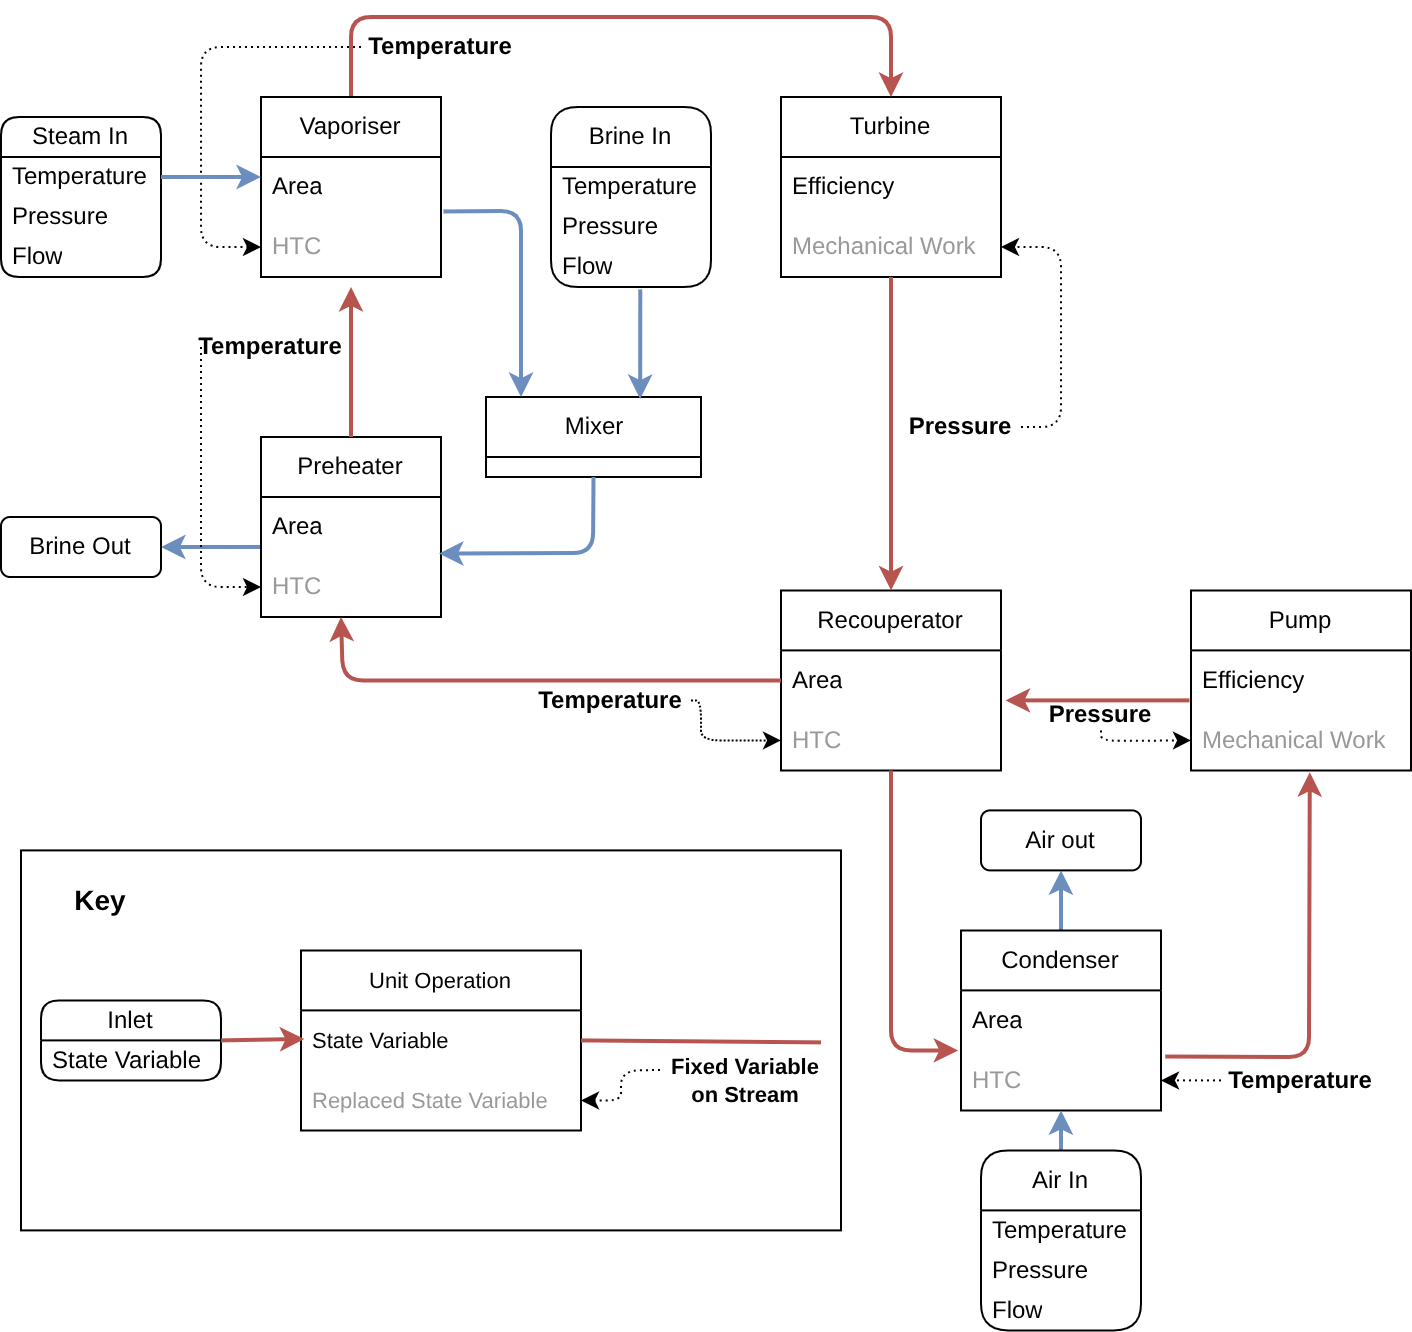
\includegraphics[width=\textwidth]{assets/geothermal-replacement.drawio.png}
\caption{Flow Diagram of a fully specified Geothermal Power Plant,
demonstrating which Canonical Variables are being replaced.}
\end{figure}

This model includes four heat exchangers
(the condenser, recouperator, preheater, and vaporiser), one turbine,
and one pump. Each of these unit operations contribute one or two
degrees of freedom: The heat exchangers need Area and Heat Transfer
Coefficient (abbreviated as HTC) to be specified, and the Turbine and
Pump both need efficiency and mechanical work. Additionally, the Steam
Inlet, Air inlet, and Brine inlet need their temperature, pressure, and
flow to be specified, as they are not connected to any upstream unit
operations.

However, the plant data includes stream pressures and temperatures, so
the mechanical work and heat transfer coefficients are not actually set
in this model. Instead, they are replaced with the pressure or
temperature measured on the stream flowing out of the unit operations.
Because of the replacement system, it is easy to see exactly why each of
these temperatures and pressures need to be specified, and why the other
streams (e.g from the recouperator to the condenser) do not need their
properties specified.

Those familiar with control systems may note that the variable
replacement approach for the pump looks similar to the control scheme of
a pump in a P\&ID Diagram, where the amount of work the pump does is
controlled by a PID tuner that reads from a pressure sensor. These are replacements that replace operating variables.
The heat exchangers are specified by their outlet temperatures, which replace the
heat transfer coefficient design variable.

We first construct the flowsheet in IDAES, the same way as any other IDAES model:

\begin{verbatim}
> m = pyo.ConcreteModel()
> m.fs = FlowsheetBlock(dynamic=False)
> m.fs.pp = iapws95.Iapws95ParameterBlock()
> m.fs.butane = build_package("helmholtz",["n-butane"],["Liq","Vap"])
\end{verbatim}

These lines:

\begin{itemize}
\tightlist
\item
  Create a new EOM in the Pyomo Framework
\item
  Add a IDAES Flowsheet into the EOM (This always required when building
  models with IDAES)
\item
  Specify the fluid property package to model water, using the IAPWS95
  specification \citep{wagner2002iapws}
\item
  Specify the fluid property package to model n-butane, using a Helmholtz
  energy formulation \citep{bucker2006reference}
\end{itemize}

Then unit models are added to the flowsheet and connected together as normal in IDAES. However,
the unit models are imported from the pyomo-replace library, which have already defined the Canonical Variables 
and appropriate initialisation methods to work with them. The models also have tagged which variables are design variables,
and which variables are operating variables.


\begin{verbatim}
> m.fs.preheater = SVHeatExchanger(hot_side={
>     "property_package": m.fs.water,
>     "has_pressure_change": False
> }, cold_side={
>     "property_package": m.fs.butane,
>     "has_pressure_change": False
> })
... continued for the rest of the flowsheet
\end{verbatim}

Arcs are also added to connect the unit models together, as normal in IDAES. 
This creates the necessary equality constraints between the variables 
on the inlet and outlet ports of the unit models.

\begin{verbatim}
> m.fs.preheater_vaporizer = Arc(
>    source=m.fs.preheater.cold_side_outlet, 
>    destination=m.fs.vaporizer.cold_side_inlet
> )
... continued for the rest of the flowsheet
\end{verbatim}

Once the unit models
have been added to the flowsheet and connected up, pyomo-replace
requires that all inlet ports are registered as Canonical Variables:

\begin{verbatim}
> register_inlet_ports(m.fs)
\end{verbatim}

This registers the properties of all inlet ports that do not have
another model upstream as state vars. This is done after the unit models
have been fully defined and any connections between unit operations have
been made. Once this method is called, the model should have zero
degrees of freedom.

Typically, at this point in a normal IDAES model, there would be many degrees of freedom and
the user would need to figure out which variables to fix to make the model square.
However, in pyomo-replace, the model is already square, and the user can simply
set values for the Canonical Variables, or replace them with other variables as required.

Pyomo-replace provides a method to print the list of Canonical Variables and any replacements that have been made:

\begin{verbatim}
> pprint_replacements(m.fs)
\end{verbatim}

This prints a list of all Canonical Variables, and any that are being
replaced by other variables. As we have not yet replaced any state
variables, it would simply print a list of all the variables that we
need to either set a value for, or replace:

\begin{verbatim}
Unreplaced state variables in block fs:
  fs.preheater.overall_heat_transfer_coefficient  (design)
  fs.preheater.area  (design)
  fs.vaporizer.overall_heat_transfer_coefficient  (design)
  fs.vaporizer.area  (design)
  fs.vaporizer._flow_mol_hot_side_inlet_ref  (inlet)
  fs.vaporizer._enth_mol_hot_side_inlet_ref  (inlet)
  fs.vaporizer._pressure_hot_side_inlet_ref  (inlet)
  fs.brine_mixer._flow_mol_inlet_2_ref  (inlet)
  fs.brine_mixer._enth_mol_inlet_2_ref  (inlet)
  fs.brine_mixer._pressure_inlet_2_ref  (inlet)
  fs.turbine.work_mechanical  (operation)
  fs.turbine.efficiency_isentropic  (design)
  fs.recuperator.overall_heat_transfer_coefficient  (design)
  fs.recuperator.area  (design)
  fs.condenser.overall_heat_transfer_coefficient  (design)
  fs.condenser.area  (design)
  fs.condenser._flow_mol_cold_side_inlet_ref  (inlet)
  fs.condenser._enth_mol_cold_side_inlet_ref  (inlet)
  fs.condenser._pressure_cold_side_inlet_ref  (inlet)
  fs.pump.work_mechanical  (operation)
  fs.pump.efficiency_pump  (design)
\end{verbatim}

This also shows which variables are tagged as design variables or operating variables.
Inlet variables are tagged separately as they don't fit neatly into either category. 
Additional categories of variables can be added if required.

We can then choose to replace any of the Canonical Variables with other variables in the model.
In this case, we want to specify the outlet conditions of the heat exchangers to calculate the appropriate
heat transfer coefficients we should design for. For numerical stability and following best practices with this property package,
we are specifying the outlet enthalpy instead of the outlet temperature. Likewise, we also specify the outlet pressure of the pump and
turbine instead of the mechanical work.
Replacing a variable is as simple as calling a function,
passing the Canonical Variable to unfix and the new variable to fix:

\begin{verbatim}
> replace_state_var(m.fs.vaporizer.overall_heat_transfer_coefficient,
                    m.fs.vaporizer.cold_side_outlet.enth_mol)
> replace_state_var(m.fs.preheater.overall_heat_transfer_coefficient,
                    m.fs.preheater.cold_side_outlet.enth_mol)
> replace_state_var(m.fs.recuperator.overall_heat_transfer_coefficient,
                    m.fs.recuperator.cold_side_outlet.enth_mol)
> replace_state_var(m.fs.condenser.overall_heat_transfer_coefficient,
                    m.fs.condenser.hot_side_outlet.enth_mol)
> replace_state_var(m.fs.pump.work_mechanical, 
                    m.fs.pump.outlet.pressure)
> replace_state_var(m.fs.turbine.work_mechanical, 
                    m.fs.turbine.outlet.pressure)
\end{verbatim}

Now we can run \texttt{pprint\_replacements} again, to show that
\texttt{work\_mechanical} has been replaced by \texttt{outlet.pressure}.

\begin{verbatim}
> pprint_replacements(m.fs)

Replacements in block fs:
(Variable -> Replaced State Var)
  fs.vaporizer._enth_mol_cold_side_outlet_ref 
      -> fs.vaporizer.overall_heat_transfer_coefficient  (design)
  fs.preheater._enth_mol_cold_side_outlet_ref 
      -> fs.preheater.overall_heat_transfer_coefficient  (design)
  fs.recuperator._enth_mol_cold_side_outlet_ref 
      -> fs.recuperator.overall_heat_transfer_coefficient  (design)
  fs.condenser._enth_mol_hot_side_outlet_ref 
      -> fs.condenser.overall_heat_transfer_coefficient  (design)
  fs.pump._pressure_outlet_ref 
      -> fs.pump.work_mechanical  (operation)
  fs.turbine._pressure_outlet_ref 
      -> fs.turbine.work_mechanical  (operation)

Unreplaced state variables in block fs:
  fs.preheater.area  (design)
  fs.vaporizer.area  (design)
  fs.vaporizer._flow_mol_hot_side_inlet_ref  (inlet)
  fs.vaporizer._enth_mol_hot_side_inlet_ref  (inlet)
  fs.vaporizer._pressure_hot_side_inlet_ref  (inlet)
  fs.brine_mixer._flow_mol_inlet_2_ref  (inlet)
  fs.brine_mixer._enth_mol_inlet_2_ref  (inlet)
  fs.brine_mixer._pressure_inlet_2_ref  (inlet)
  fs.turbine.efficiency_isentropic  (design)
  fs.recuperator.area  (design)
  fs.condenser.area  (design)
  fs.condenser._flow_mol_cold_side_inlet_ref  (inlet)
  fs.condenser._enth_mol_cold_side_inlet_ref  (inlet)
  fs.condenser._pressure_cold_side_inlet_ref  (inlet)
  fs.pump.efficiency_pump  (design)
\end{verbatim}

Then a value can be specified for all the variables that are replacing Canonical Variables, and all the Canonical Variables that
have not been replaced. This model can then be initialized and solved using the standard pyomo and idaes
libraries.

To switch this model from a design case to a performance rating case, we can simply remove the replacements on the design variables:

\begin{verbatim}
deactivate_category(m.fs, "design")
\end{verbatim}

This re-fixes the heat exchanger overall heat transfer coefficients, 
but keeps the replacements on the operating variables. This is scalable to larger models, as the design variables are tagged ahead of time,
meaning that it is always easy to switch between these cases. Because of the coupling between design variables and their replaced variables, the model includes
information about which dependent variables need to be removed when the design variables are fixed again.

To switch the model to a ``simulation" case, where all design and operating variables are fixed, we can also remove the replacements on the operating variables.
This will revert to the original set of initial variables. Thus, it becomes easy to use the model for a variety of use cases, as variable replacement and the tagging of the design and operating variables provides the additional metadata required.

\hypertarget{dynamic-tank}{%
\subsection{Dynamic Tank}\label{dynamic-tank}}

\begin{figure}
\centering
\includegraphics[width=\textwidth]{assets/dynamics.drawio.png}
\caption{A model of a tank with valves controlling the inlet and the
outlet. Properties with an asterisk (*) next to them are not
time-indexed. The tank outlet pressure is referenced by the PID
controller, but is not a Canonical Variable.}
\end{figure}

A dynamic flowsheet allows us to test a different aspect of our system:
how indexed variables are handled. In this flowsheet, we have a steam
tank, modelled as a Heater in idaes, with a constant volume and an inlet
and outlet valve controlling the flow rate in and out of the tank. The
flow into the tank is controlled by a PID controller, which is targeting
a certain outlet pressure within the tank.

Both the valves have two Canonical Variables: the valve coefficient, and the
valve opening fraction. However, the valve coefficient is a constant
property; it cannot be changed throughout the simulation. To indicate
this, we have included an asterisk (*) next to them. In contrast, the
valve opening fraction can be changed over time, and so in IDAES it is
indexed by time. It is actually a set of variables, one variable for
every time step across the simulation. Variables with an asterisk next
to them cannot replace variables without an asterisk and vice versa,
because the time indexed variables actually represent many degrees of
freedom, while the others only represent one degree of freedom. However,
in almost all cases it makes sense to treat the variable across time in
the same manner (either you want to fix it, or you don't.)

In this flowsheet, only two replacements are required. The first
involves replacing the inlet flow with the outlet pressure. These can be
replaced because a pressure difference between the inlet and the outlet
is what drives the fluid through the system. The flow can be calculated
from the valve pressure-flow correlation. Both pressure and flow are
time-indexed properties, so they each represent the same number of
degrees of freedom. Note that with our initialisation strategy, we start
with a guess for flow, and then we initialise with that. After
initialisation is completed, the flowsheet re-solves with the correct
outlet pressure fixed, recalculating what the true flow value is.

The second replacement involves replacing the valve opening fraction
with the setpoint. The PID controller sets the value of the valve
opening fraction, so the valve opening fraction no longer needs to be
specified. This goes against the general logic of variable replacement.
However, the setpoint of the PID controller needs to be specified. So we
can add a replacement to say that the setpoint replaces the valve
opening fraction. This is a simple solution that can be done when the
PID controller is connected up to the valve opening fraction.

Initial Material Accumulation and Initial Energy Accumulation can be
treated as additional Canonical Variables if it is appropriate. It would be
feasible to use the replacement logic to replace them with Initial
Material Holdup and Initial Energy Holdup. However, typically dynamic
flowsheets start with a steady-state assumption, and all accumulation
terms are fixed to zero.

This case study successfully demonstrates that the variable replacement
logic can easily be extended to more complex flowsheet scenarios
involving dynamics or other indexed variables.

\hypertarget{ahuora-digital-twin-platform}{%
\subsection{Ahuora Digital Twin
Platform}\label{ahuora-digital-twin-platform}}

\begin{figure}
\centering
\includegraphics[width=\textwidth]{assets/ahuora-interface.png}
\caption{A Heat pump in the Ahuora Platform.}
\end{figure}

While this paper has focused on the theoretical advantages of a Variable
Replacement methodology, a major reason we have developed this method of
variable replacement is because it works particularly well in a
graphical user interface.

The Ahuora Digital Twin Platform is a web-based process simulation
environment. It is built using IDAES and Pyomo as the equation-oriented
modelling libraries as the simulation backend.

Each unit operation has a set of Canonical Variables, where the user can
enter a value, and a set of calculated variables, which cannot be
entered by the user. If a user wants to fix a calculated variable, an
appropriate Canonical Variable has to be chosen and ``replaced''. This makes
the Canonical Variable a ``guess'': the user still needs to enter a value,
but it is shown with no background color, to indicate to the user that
it will be calculated when the flowsheet is solved. A message tells the
user what variable is replacing it. The calculated variable then becomes editable.
A message shows which variable it is
replacing,  ensures the user is able to keep track of replacements.

\begin{figure}
\centering
\includegraphics[width=\textwidth]{assets/ahuora-replacement.png}
\caption{Variable replacement on a Compressor model in the Ahuora
Platform.}
\label{fig:ahuora-replacement}
\end{figure}

In \cref{fig:ahuora-replacement}, the ``Isentropic Efficiency'' Canonical Variable is fixed at approximately 70\%. 
The ``Mechanical Work'' Canonical Variable in the Compressor is being
replaced by the Pressure at the outlet stream. An initial guess for
``Mechanical Work'' may still be entered, which is updated to the
correct value, which is based on the pressure specified at the outlet,
when the model solves.

Before using the variable replacement approach, we only limited the user
to a fixed set of choices of variables for each unit operation. However,
this reduced functionality significantly as there was no method to
specify unit models indirectly, such as through downstream properties.
We thought about trying a degrees of freedom approach, but were
concerned that it would be much too confusing as it didn't provide the
user with any direction on how to get started.

One of the major advantages of Variable Replacement that we have noticed
in a GUI is that it provides additional context for unit operations. In
a GUI program, it is very easy to visually show that context by
styling fixed Canonical Variables, guesses, and calculated variables
differently, and to show the links between variables.

Working with a GUI also means that adding and removing unit operations
is common, and Variable Replacement provides a sensible way to deal with
adding or removing unit operations. When a unit operation is added, it's
Canonical Variables and inlet ports are fixed by default to ensure the
degrees of freedom are still zero. When a unit operation is removed,
anything that is replacing its Canonical Variables is also unfixed, and any
inlet ports that were previously connected to the outlet of the unit
operation are fixed, again keeping the degrees of freedom at zero.

The GUI also does not provide any way to write custom initialisation
routines, because these are usually specified as python code and can be
quite complex, so it is out of scope of the project. However, the
multi-stage initialisation that naturally works with variable
replacement helps to improve the reliability of solving. As guesses are
specified for the Canonical Variables, these can be used in the
initialisation routine. In particular, this enables us to specify any
set of variables to define the conditions of an inlet stream, whereas
IDAES does not have initialisation routines for any set of state
variables and is typically limited to only a certain set of properties.













\hypertarget{properties-of-a-variable-replacement-approach-to-equation-oriented-modelling}{%
\section{Discussion}\label{properties-of-a-variable-replacement-approach-to-equation-oriented-modelling}}

This method of replacing Canonical Variables does not fundamentally change
the underlying model equations, solver, or structural analysis.
Technically, it is still based on fixing one variable and unfixing
another. The contribution is that this action is elevated into an
explicit specification-management layer that records intent, preserves
consistency, and makes specification changes easier to interpret and
automate.

A useful analogy may be in the study of programming language theory.
Functional and Imperative programming languages are both turing
complete, but certain problems are better represented in an imperative
language, while other problems are more simply expressed in a functional
manner. Likewise, static typing systems do not change the correctness of
a program, but they do make it simpler to validate and reason about the
program.

Variable replacement enforces a degree of regularity in the blocks that
make up models, and in the overall structure. In that sense, it offers
a more structured way to reason about specification topology in
equation-oriented systems.

\begin{enumerate}
\def\labelenumi{\arabic{enumi}.}
\tightlist
\item
  It reduces the manual burden of Degrees of Freedom management when
  defining and modifying a model.
\item
  Switching between different types of analysis for design versus
  operation becomes easier.
\item
  It standardises initialisation routines, as long as guesses are
  provided for Canonical Variables.
\item
  The coupling of variables adds a level of interpretability to the
  model's specification, which makes it easier to maintain and
  manipulate models.
\end{enumerate}

\hypertarget{removing-the-problem-of-squaring-a-model}{%
\subsection{Reducing the manual burden of squaring a
model}\label{removing-the-problem-of-squaring-a-model}}

To have a square model, you must have the same number of unknowns, or
unfixed variables, as equations, i.e
\(n_{\text{degrees\ of\ freedom}} = 0\).

Traditional model libraries such as IDAES provide the equations, and
then all that is required is to specify enough variables that the number
of variables equals the number of unknowns. This can be done by
repeatedly fixing variables in a part of a model that is not already
over-defined\footnote{i.e You must fix variables that are part of a
  Dulmage-Mendelson under-constrained set.}, until the model is fully
defined. Incorrect degrees of freedom has been identified as a common
source of errors in EOMs, and checking the degrees of freedom is the
first recommended step to diagnose problems \citep{lee2024model}. Newer
analysis methods, such as Dulmage-Mendelson Decomposition do make this
simpler, but it is still an iterative process.

Using a Variable Replacement approach, a set of Canonical Variables would
already be defined by the model library, so the user would not need to
manually square the baseline model. There are zero degrees of freedom
\emph{by construction} for that baseline specification. If a problem
requires a variable to be fixed that is not a Canonical Variable, an
appropriate\footnote{i.e a Canonical Variable that would be part of the
  Dulmage-Mendelson over-constrained set if the other variable was
  fixed and nothing was unfixed} Canonical Variable must be unfixed too.
Because the workflow requires adding and removing one specification
together, it preserves a square model through the replacement process.
In practice this removes much of the trial-and-error associated with
manual specification changes in EOMs.

\hypertarget{switching-between-different-types-of-analysis}{%
\subsection{Switching between different types of
analysis}\label{switching-between-different-types-of-analysis}}

We have previously discussed using the car example that some state
variables are design Canonical Variables (i.e \(k\)), and some are
manipulated variables (i.e \(y\)), and all other variables are dependent
(i.e \(v\)).

A design problem would involve finding an appropriate value for the design
Canonical Variables, by calculating a desired \(k\). In an operation case,
\(k\) is fixed and known, but an appropriate value of \(y\) may be
required. To turn a design case into an operation case, all that is
required is to fix all the design variables, which can be done un-doing
any replacements that have happened on them. With the additional
metadata on what variables are replacing what, it becomes much easier to
create tools to switch between design and operation modes.

Likewise, a robustness test typically involves fixing only the decision
variables (both design and operation) and calculating how sensitive the
dependent variables are to changes. Again, this is easy to do in the
variable replacement framework by simply undoing all replacements, as
the decision variables are the Canonical Variables.

\hypertarget{simplified-initialisation}{%
\subsection{\texorpdfstring{Simplified Initialisation
}{Simplified Initialisation }}\label{simplified-initialisation}}

Initial guesses greatly increase the robustness of solving EOMs.
Modelling toolboxes such as IDAES provide methods to automatically
define initial guesses based on fixed variables. However, if different
variables are fixed to the ones the modelling library expects, these
methods will not provide any benefit, and may even cause additional
problems.

\begin{figure}
\centering
\includegraphics[width=\textwidth]{assets/initialisation-methods.drawio.png}
\caption{Alternative initialisation routine, making use of state
variables to avoid the need for different initialisation methods.}
\end{figure}

The concept of ``Canonical Variables'' can simplify this process, by
splitting the initialisation into two parts. First, the initialisation
methods can calculate initial values of all variables based on the
values or guesses of the Canonical Variables. Then, once the model has been
initialised in a sensible location, any Canonical Variables that are
replaced (i.e, were guesses) can be unfixed, and the variables that are
replacing them can be fixed back to their original values. The block can
then be re-solved to calculate the correct value of any ``guessed''
Canonical Variable.

This limits the logic in initialisation routines, as only one
initialisation method is required be required. It does require that
initial guesses are provided for all the Canonical Variables, but this is a
reasonable tradeoff. This standardises the initialisation process to
work across all sets of fixed variables, while still giving the model
library developer freedom to develop whatever initialisation method they
think is best.

A test with the IDAES turbine model demonstrates this to be the case. A
turbine model was constructed, with 100 mol/s of 200~$^\circ$C steam at 1 MPa, an
isentropic efficiency of 50\% and a pressure drop of 900 kPa. Different
combinations of variables were fixed, and then the model was initialised
and then solved with those fixed variables using IDAES's standard
initialisation routines. Idaes's initialisation routines check which
variables are fixed and perform different initialisation methods
accordingly.

This was compared to the same model, at the same conditions, but with
initialisation performed first using a guess for efficiency and work.
Subsequently, efficiency and work are unfixed and the model is solved
using the specified variables.

\begin{longtable}[]{@{}lll@{}}
\caption{Comparison of solving success with different combinations of
variables, with and without staged initialisation.}\tabularnewline
\toprule
\begin{minipage}[b]{0.19\columnwidth}\raggedright
Fixed Variables\strut
\end{minipage} & \begin{minipage}[b]{0.36\columnwidth}\raggedright
Standard IDAES Initialisation\strut
\end{minipage} & \begin{minipage}[b]{0.37\columnwidth}\raggedright
Staged Initialisation Approach\strut
\end{minipage}\tabularnewline
\midrule
\endfirsthead
\toprule
\begin{minipage}[b]{0.19\columnwidth}\raggedright
Fixed Variables\strut
\end{minipage} & \begin{minipage}[b]{0.36\columnwidth}\raggedright
Standard IDAES Initialisation\strut
\end{minipage} & \begin{minipage}[b]{0.37\columnwidth}\raggedright
Staged Initialisation Approach\strut
\end{minipage}\tabularnewline
\midrule
\endhead
\begin{minipage}[t]{0.19\columnwidth}\raggedright
Mechanical Work \& Efficiency\strut
\end{minipage} & \begin{minipage}[t]{0.36\columnwidth}\raggedright
Success\strut
\end{minipage} & \begin{minipage}[t]{0.37\columnwidth}\raggedright
Success\strut
\end{minipage}\tabularnewline
\begin{minipage}[t]{0.19\columnwidth}\raggedright
Work \& Outlet Pressure\strut
\end{minipage} & \begin{minipage}[t]{0.36\columnwidth}\raggedright
Initialisation Error\strut
\end{minipage} & \begin{minipage}[t]{0.37\columnwidth}\raggedright
Success\strut
\end{minipage}\tabularnewline
\begin{minipage}[t]{0.19\columnwidth}\raggedright
Efficiency \& Outlet Pressure\strut
\end{minipage} & \begin{minipage}[t]{0.36\columnwidth}\raggedright
Success\strut
\end{minipage} & \begin{minipage}[t]{0.37\columnwidth}\raggedright
Success\strut
\end{minipage}\tabularnewline
\begin{minipage}[t]{0.19\columnwidth}\raggedright
Work \& Pressure Ratio\strut
\end{minipage} & \begin{minipage}[t]{0.36\columnwidth}\raggedright
Initialisation Error\strut
\end{minipage} & \begin{minipage}[t]{0.37\columnwidth}\raggedright
Success\strut
\end{minipage}\tabularnewline
\begin{minipage}[t]{0.19\columnwidth}\raggedright
Efficiency \& Pressure Ratio\strut
\end{minipage} & \begin{minipage}[t]{0.36\columnwidth}\raggedright
Success\strut
\end{minipage} & \begin{minipage}[t]{0.37\columnwidth}\raggedright
Success\strut
\end{minipage}\tabularnewline
\bottomrule
\end{longtable}

\hypertarget{interpretability-and-model-maintenance.}{%
\subsection{Interpretability and model
maintenance.}\label{interpretability-and-model-maintenance.}}

In conventional programming languages, type systems are frequently used
to increase a programs interpretability. In many cases, typing is not
strictly necessary for a program to run, but it bakes in crucial context
about what the expected inputs and outputs of a piece of code are. While
this is generally more verbose than the equivalent untyped code, many
developers find this invaluable in helping to understand the system.

The replacement system works in a similar manner, as it bakes in more
context to the model. Similar to a type system in a programming
language, this increases the model's interpretability and
maintainability. Technically, it doesn't matter which Canonical Variable a
model is replacing; just which variables are fixed and which are
unfixed. However, having that context makes understanding \emph{why} a
variable needs to be fixed much clearer.

Admittedly, interpretability is a subjective concept. Thus it will be
illustrated through a series of examples differing in scale and
complexity, and reasoning will be provided as to why the extra context
that Variable Replacement provides benefits that case.

\hypertarget{example-1-a-single-compressor}{%
\subsubsection{Example 1: A single
Compressor}\label{example-1-a-single-compressor}}

A simple compressor model, using a traditional modelling toolbox, may
include the following variables as shown in Figure \ref{compressor-dof}.

\begin{figure}
\centering
\includegraphics[width=\textwidth]{assets/compressor-5dof.drawio.png}
\caption{Variables in a simple compressor model. \label{compressor-dof}}
\end{figure}

The equivalent model, using a variable replacement approach, would have
Canonical Variables already defined by the developer of the Compressor Unit
Model (Figure \ref{compressor-sv-defined}).

\begin{figure}
\centering
\includegraphics[width=\textwidth]{assets/compressor-sv.drawio.png}
\caption{Variables in a simple compressor model, with everything that is
not a fixed greyed out. \label{compressor-sv-defined}}
\end{figure}

This is more interpretable, as it provides extra context: it explains
what the model developer expected was most likely to be fixed.

However, depending on the problem, different variables may be fixed. For
example, the outlet pressure may be known instead of the mechanical
work. In a degree-of-freedom based modelling system, the user would just fix the outlet pressure
instead of the mechanical work (Figure
\ref{compressor-fixed-traditional}).

\begin{figure}
\centering
\includegraphics[width=\textwidth]{assets/compressor-fixed-outlet.drawio.png}
\caption{Fully specified compressor model using a traditional approach.
\label{compressor-fixed-traditional}}
\end{figure}

Using a variable replacement approach, the user must explicitly replace 
the mechanical work Canonical Variable with the outlet pressure. This
would create a link between the two variables to show what Mechanical
work was replaced by (Figure \ref{compressor-replacement}).

\begin{figure}
\centering
\includegraphics[width=\textwidth]{assets/compressor-replaced.drawio.png}
\caption{Compressor model using the variable replacement system, with
Outlet Pressure replacing Mechanical Work.
\label{compressor-replacement}}
\end{figure}

This provides a natural form of documentation for the model: The outlet
pressure is being specified because it is needed to calculate the
mechanical work of the compressor. On large systems, this explanation
becomes particularly beneficial, as it becomes harder to identify why a
property needs to be set, particularly when degrees of freedom are being
specified indirectly.

\hypertarget{example-2-modifying-a-flowsheet}{%
\subsubsection{Example 2: Modifying a
flowsheet}\label{example-2-modifying-a-flowsheet}}

EOMs are generally evaluated when they are complete, and their evolution
and development is ignored. However, in practice EOMs are built like
pieces of software; iteratively and incrementally over time\footnote{A
  good explanation of iterative vs incremental development is discussed
  by Jeff Patton at
  \url{https://jpattonassociates.com/dont_know_what_i_want/}}. A model
is generally built by applying a series of modifications to a simple
model, including:

\begin{itemize}
\tightlist
\item
  Changing which variables are fixed (In variable replacement, this
  would be replacing variables, in a Degrees of freedom approach, this
  would be fixing and unfixing variables)
\item
  Adding a new variable with a corresponding constraint to define it
  (e.g defining a custom calculated property)
\item
  Adding a new set of variables and corresponding constraints (e.g
  adding an additional unit operation to a model)
\item
  Replacing a constraint or set of constraints with an alternative
  specification (e.g switching to a different formulation of a compound
  or unit operation's characteristics)
\item
  Removing a set of variables and/or constraints from a model (e.g
  removing a unit operation that is not required in a model)
\item
  Replacing a fixed variable with a constraint to define that variable.
\end{itemize}

Because the number of unfixed variables must always be the same as the
number of constraints, when unfixed variables are added or removed, the
same number of constraints need to be added or removed too. However,
this is a non-trivial process. If a variable is removed, which
constraint should be removed with it? This problem compounds when you
are removing multiple variables and constraints simultaneously.

\begin{figure}
\centering
\includegraphics[width=\textwidth]{assets/deleting-replacement.drawio.png}
\caption{Deleting the pump from a flowsheet is handled elegantly as the
fixed variables are coupled to specific Canonical Variables.}
\end{figure}

Consider this model of a pump connected to a heater, with all the state
variables defined. The inlet conditions are Canonical Variables, and so is
the mechanical work of the pump, and the heat duty of the heater.
However, the mechanical work and heat duty are replaced by the
temperature and pressure of the outlet; i.e the temperature and pressure
will be used to calculate mechanical work and heat duty.

When the pump is removed from the flowsheet, the intermediate stream
becomes the new inlet, and thus its temperature, pressure, and flow will
need to be fixed. Because the outlet pressure was replacing Mechanical
Work on the pump, and the pump has been removed, outlet pressure no
longer needs to be fixed. Thus, the model is still fully specified.

Defining which variables are design variables and which variables are 
operating variables further improves this process, allowing a user
to easily switch the model between completely different analysis modes.

\begin{figure}
\centering
\includegraphics[width=\textwidth]{assets/deleting-traditional.drawio.png}
\caption{Using a traditional EOM modelling methodology, there is no coupling
of variables, so when the pump is deleted there is no intuition what
variables to remove.}
\end{figure}

Using a traditional EOM modelling methodology, there is no coupling of
variables, so when the pump is deleted there is no information provided
on what variables to remove. There are two options:

\begin{enumerate}
\def\labelenumi{\arabic{enumi}.}
\tightlist
\item
  Fix the inlet conditions automatically, similar to the strategy in
  variable replacement. This will leave you with an over-defined model,
  as pressure would still be fixed on the outlet also. The modeller
  would have to manually unfix outlet pressure to again have a solvable
  model.
\item
  Don't fix the inlet conditions automatically. This would leave you
  with an under-defined model, and the modeller would have to choose two
  variables to fix (e.g inlet temperature and flow) to again have a
  solvable model.
\end{enumerate}

Both of these options require manual intervention from the modeller, as
there is no clear path to maintain a solvable model. In comparison, when
fixed variables are coupled to a set of Canonical Variables, it is easy to
see when to unfix the variable: when the state var it is connected to is
removed.

\hypertarget{analysing-interpretability}{%
\subsubsection{Analysing
interpretability}\label{analysing-interpretability}}

Whether the method of replacement improves interpretability and
maintainability is a subjective question. Nonetheless, these examples
demonstrate the basic properties of Variable Replacement, and the
advantages that it can provide in understanding the relationships
between fixed variables in the system, without needing to dig into the
underlying mathematical formulations. This also makes it simpler to
modify a model and maintain a solvable state. However, similar to typed
languages in software development, the realisable benefit may depend on
the use case.


\hypertarget{conclusion}{%
\section{Conclusions}\label{conclusion}}

Variable replacement provides an alternative way of maintaining a square
model in an equation-oriented framework, particularly when scaling up to
larger EOMs.

If Canonical Variables are defined on each block added to a model, those who
use the model do not need to first square the problem. Degrees of
freedom are kept at zero through any changes that are made to the
flowsheet. The coupling between Canonical Variables and fixed variables
provides a more interpretable way of reasoning about the model, bringing
the relationships between variables to the forefront. Tagging Canonical Variables
with metadata about their real-world meaning, such as if they are design parameters 
or operating parameters, makes it easy to switch between different use cases.
Additionally, enforcing a standard set of Canonical Variables and requiring the user
to provide initial guesses for them makes it simpler to
build initialisation and scaling methods. The Ahuora Digital Twin
Platform provides a case study on how this is beneficial, particularly
when using a GUI tool for modelling.

While this paper introduces Variable Replacement as a method and preview
its potential benefits in the chemical engineering domain, further research is required to systematically
evaluate the interpretability and initialisation advantages across
different types of EOMs. Nonetheless, these techniques hold promise to
standardise the creation and use of libraries of EOMs. This would enable
equation-oriented modelling to be used in a more maintainable way on
large projects, such as Process Digital Twins, in the future.

\newpage
